\providecommand{\zZ}{\hskip 3.6pt plus1.2pt minus0.8pt}
\providecommand{\McQ}{\fontfamily{cwM}\fontseries{2}\selectfont}
\providecommand{\MbQ}{\fontfamily{cwM}\fontseries{1}\selectfont}
\providecommand{\zz}{\hskip 0.6pt plus0.2pt minus0.1pt\ignorespaces}
\providecommand{\MdQ}{\fontfamily{cwM}\fontseries{3}\selectfont}
\catcode+252=1 \catcode+253=2 \catcode+254=0 \catcode+251=4
\providecommand{\MmQ}{\fontfamily{cwM}\fontseries{12}\selectfont}
\providecommand{\z}{\hskip 0.0pt plus0.2pt minus0.1pt}
\providecommand{\Z}{\hskip 1.2pt plus0.4pt minus0.2pt}
\providecommand{\cH}{\char}
\providecommand{\MjQ}{\fontfamily{cwM}\fontseries{9}\selectfont}
\documentclass[a4paper,12pt]{article}
\usepackage{ amssymb }
\usepackage{ stmaryrd }
\usepackage{ dsfont }
\usepackage{amsmath}
\usepackage{mathtools} 
\newcommand{\tabincell}[2]{\begin{tabular}{@{}#1@{}}#2\end{tabular}} %{\McQ\cH91}{\MbQ\cH143}{\MaQ\cH113}{\MbQ\cH35}{\MaQ\cH132}{\MfQ\cH178}{\McQ\cH87}{\MaQ\cH223}{\MbQ\cH224}
\usepackage{textcomp}
\renewcommand{\baselinestretch}{1.5} % 5 linespace
%\usepackage{MinionPro} %{\MiQ\cH28}{\MfQ\cH220}{\MiQ\cH116}{\MbQ\cH143}{\MbQ\cH61}{\MbQ\cH224}{\MbQ\cH237}{\McQ\cH76}{\MbQ\cH100}{\MbQ\cH98}{\MaQ\cH229}{\MaQ\cH229}{\McQ\cH241}
\usepackage[utf8]{inputenc}
\usepackage{geometry}
\usepackage{graphicx,psfrag,booktabs}
\geometry{left=1in,right=1in,top=1in,bottom=1in}
\usepackage{graphicx}
\usepackage{titlesec}
\titlelabel{\thetitle.\quad} %{\MaQ\cH94}{\MbQ\cH90}section {\McQ\cH41}{\McQ\cH85}{\MbQ\cH237}{\MeQ\cH165}{\MdQ\cH168}
\usepackage{mathrsfs} %{\MaQ\cH139}{\MaQ\cH112}{\McQ\cH73}{\McQ\cH241}{\MaQ\cH229}{\MgQ\cH130}{\MeQ\cH165}{\MdQ\cH168}
%\usepackage{indentfirst}%{\McQ\cH199}{\McQ\cH229}{\McQ\cH11}{\MaQ\cH115}{\MbQ\cH143}{\MbQ\cH237}{\MbQ\cH78}{\MaQ\cH73}
\usepackage[square,numbers]{natbib}
\usepackage{xeCJK} %{\MaQ\cH50}{\MbQ\cH100}{\MaQ\cH229}{\McQ\cH241}{\McQ\cH113}{\MaQ\cH236}
\setCJKmainfont{SimSun} %{\McQ\cH227}{\McQ\cH113}{\MaQ\cH53}{\MaQ\cH50}{\MbQ\cH100}{\MaQ\cH229}{\McQ\cH241}
\bibliographystyle{unsrtnat}
\makeatletter
\def\@xfootnote[#1]{%
  \protected@xdef\@thefnmark{#1}%
  \@footnotemark\@footnotetext}
\makeatother

\title{Home Work 3\\ Machine Learning Foundations}
\author{R04323050 \\{\McQ\cH37}\z{\MbQ\cH200}\z{\MmQ\cH238}\z{\McQ\cH250}   \quad {\McQ\cH207}\z{\MdQ\cH43}\z{\MjQ\cH254}}
\date{}

\begin{document}
\maketitle
\section{}
\begin{figure}[h]
\centering
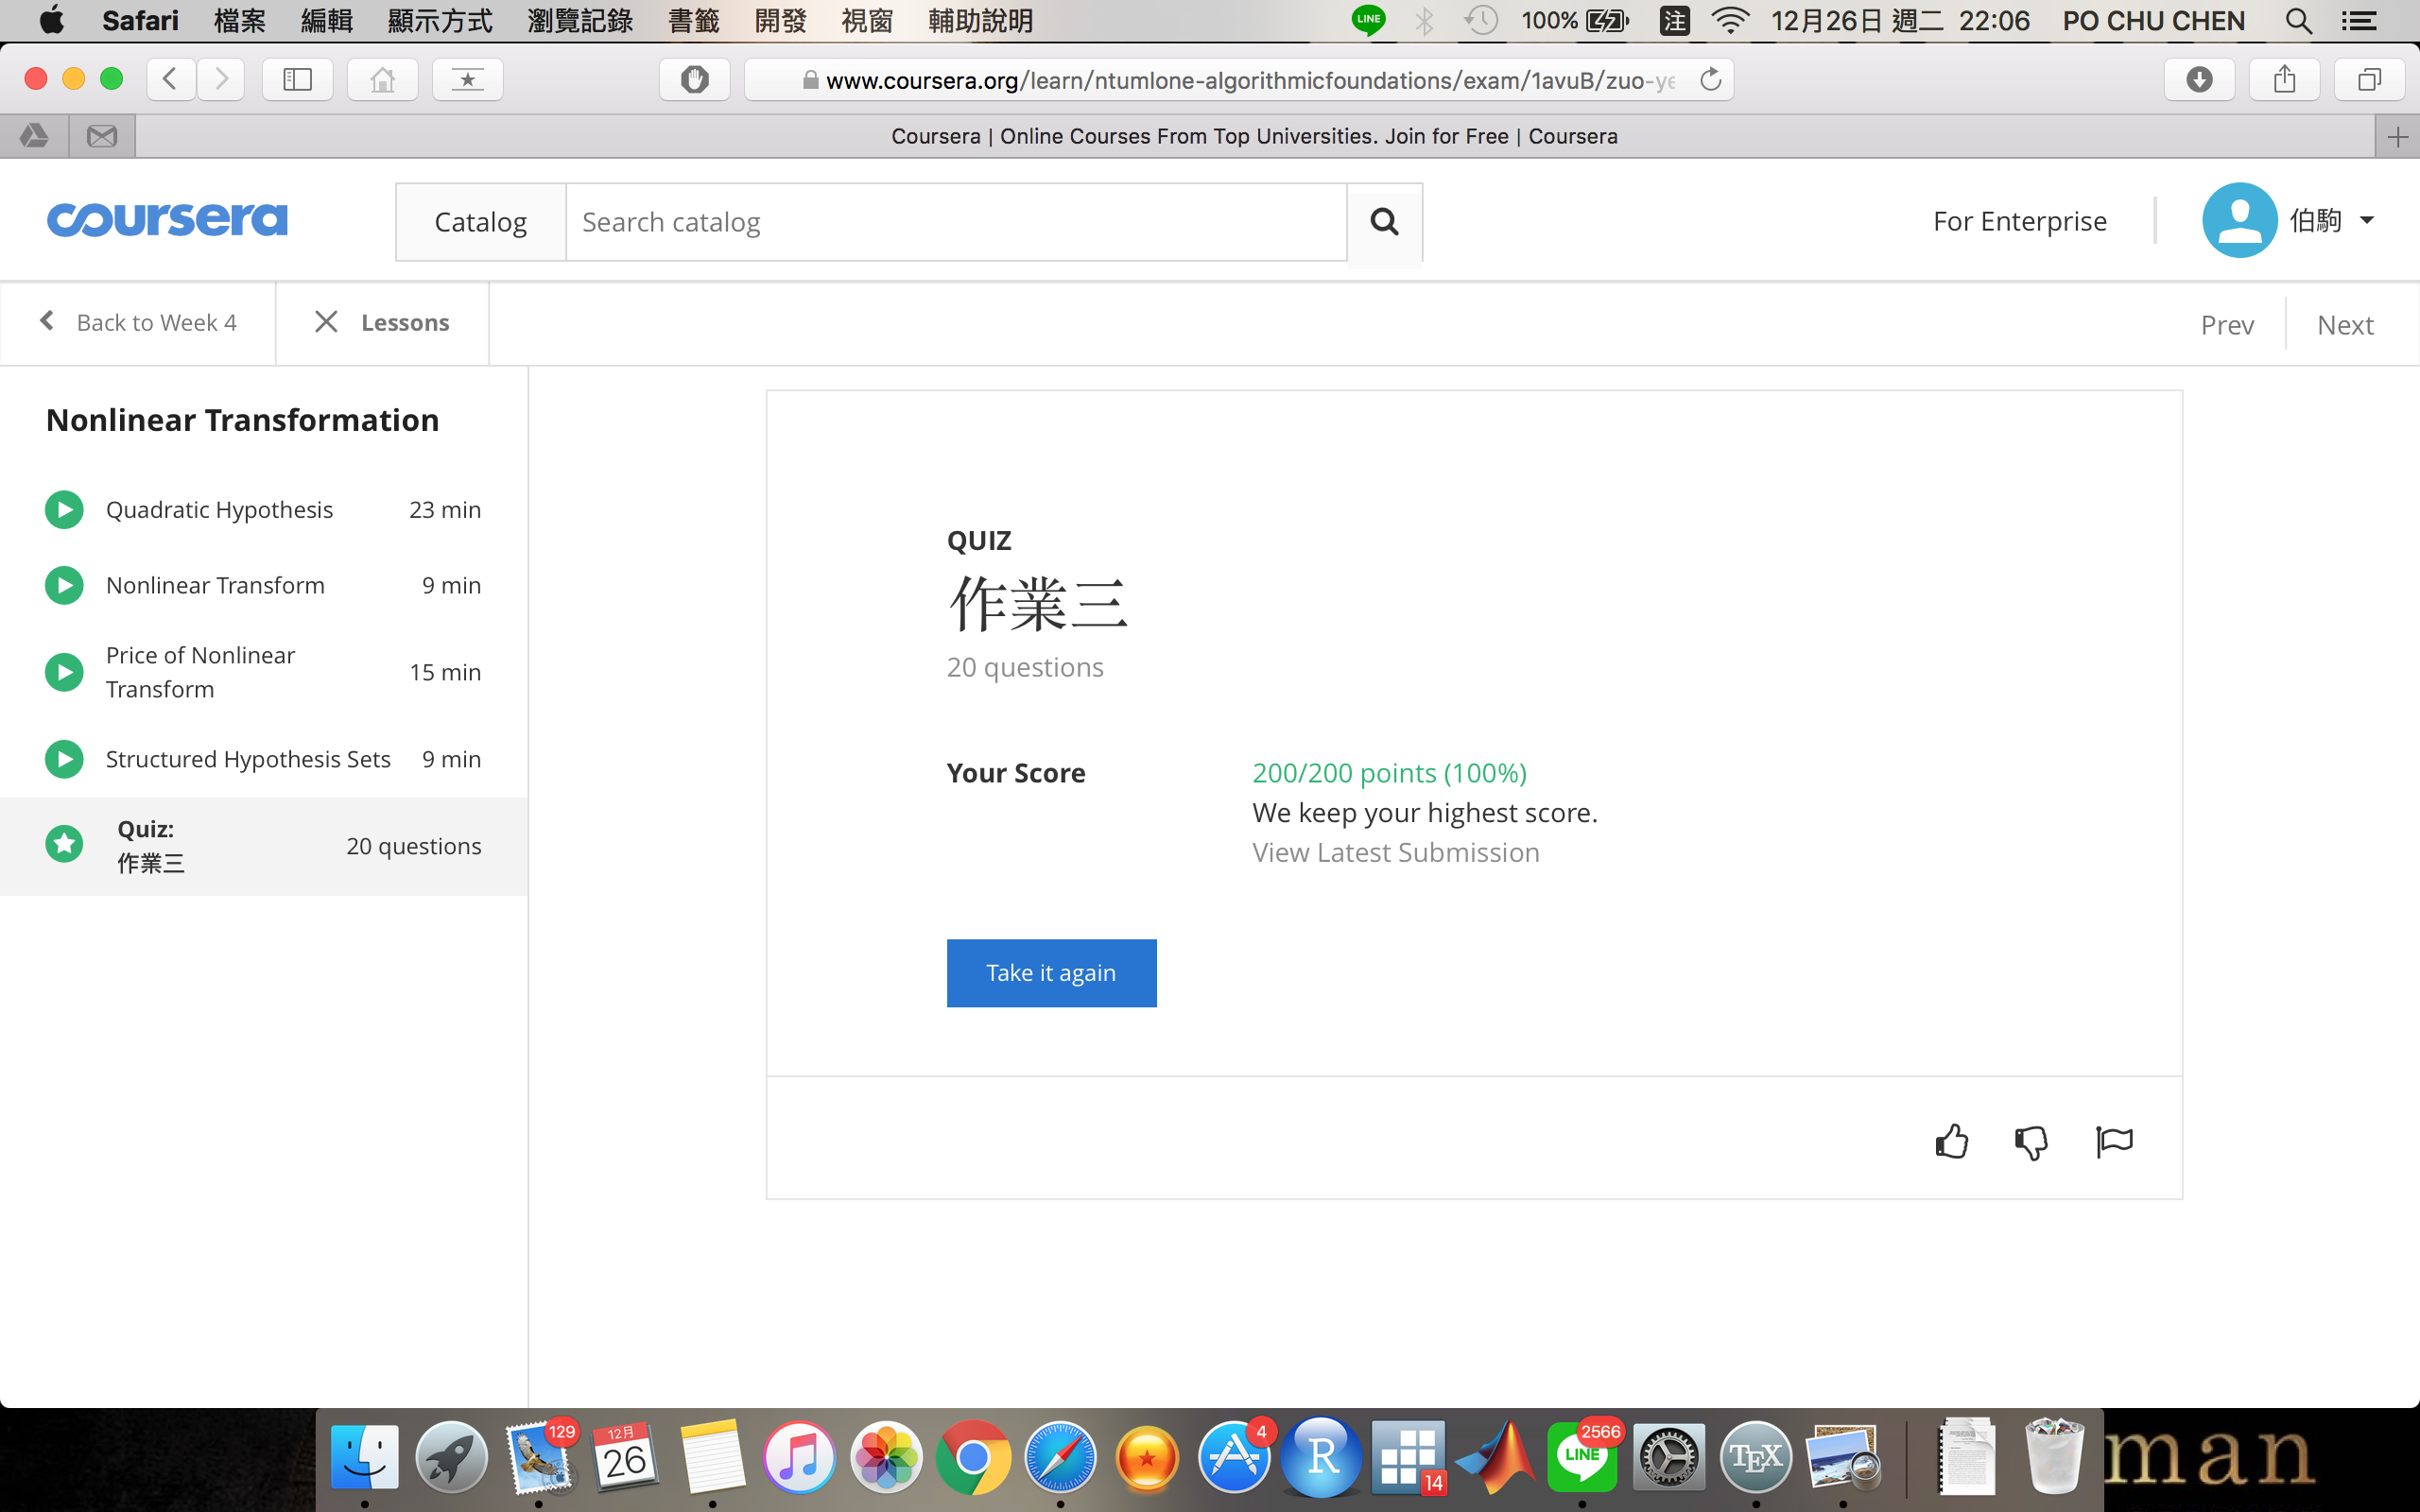
\includegraphics[scale=0.3]{Q1.png}
\end{figure}

\section{}
\textbf{\underline{Claim:}} $(I-H)$ is idempotent. i.e $(I-H)^2=(I-H)$, where $H=\mathbf{X}(\mathbf{X}^{T}\mathbf{X})^{-1}\mathbf{X}^{T}$ \\

\begin{align*} 
H=\mathbf{X}(\mathbf{X}^{T}\mathbf{X})^{-1}\mathbf{X}^{T}, \quad H \cdot H&=\mathbf{X}(\mathbf{X}^{T}\mathbf{X})^{-1}\mathbf{X}^{T} \cdot \mathbf{X}(\mathbf{X}^{T}\mathbf{X})^{-1}\mathbf{X}^{T} \\
&= \mathbf{X}(\mathbf{X}^{T}\mathbf{X})^{-1}(\mathbf{X}^{T}  \mathbf{X})(\mathbf{X}^{T}\mathbf{X})^{-1}\mathbf{X}^{T} \\
&= \mathbf{X}(\mathbf{X}^{T}\mathbf{X})^{-1} I \mathbf{X}^{T} \\
&= \mathbf{X}(\mathbf{X}^{T}\mathbf{X})^{-1} \mathbf{X}^{T} = H \\
\text{Hence},\quad  (I-H)^2 &= (I-H) \cdot (I-H) \\
&= I(I-H) - H(I-H) = I-H-H+H \cdot H \\
&= I-2H+H = I-H 
\end{align*}

\section {}
$err(\mathbf{w})=\text{max}(0, -y\mathbf{w}^{T}\mathbf{x})$, W.L.O.G. let $y=1$ \\
\textcircled{1} $\mathbf{w}^{T}\mathbf{x}<0, \, err(\mathbf{w})=-y\mathbf{w}^{T}\mathbf{x}, \nabla_{\mathbf{w}} err(\mathbf{w})=-y\mathbf{x}, \, y \neq sgn(\mathbf{w}^{T}\mathbf{x})$   \\
\textcircled{2} $\mathbf{w}^{T}\mathbf{x}>0, \, err(\mathbf{w})=0, \nabla_{\mathbf{w}} err(\mathbf{w})=0, \, y = sgn(\mathbf{w}^{T}\mathbf{x})$ \\
Plugging the formula of SGD: $\mathbf{w}_{t+1} \leftarrow \mathbf{w}_{t} + \eta \cdot (-\nabla_{\mathbf{w}} err(\mathbf{w}))$ \\
Let $\eta=1$, then $\mathbf{w}_{t+1} \leftarrow \mathbf{w}_{t}-\nabla_{\mathbf{w}} err(\mathbf{w}) = \mathbf{w}_{t} + \llbracket y \neq sgn(\mathbf{w}^{T}\mathbf{x})\rrbracket \cdot (y\mathbf{x})$ \\
It's obvious that the above result is a PLA iteration in P.11 of slides 11.

\section{}
Given $\widehat{E_{2}}(\Delta u, \Delta v)$ is the second-order Taylor's expansion of $E(u,v)$. \\
$\widehat{E_{2}}(\Delta  u, \Delta v)= E(u,v) + \begin{bmatrix}\frac{\partial E}{\partial u} & \frac{\partial E}{\partial v}\end{bmatrix} \begin{bmatrix}\Delta u\\ \Delta v \end{bmatrix} + \frac{1}{2} \begin{bmatrix} \Delta u& \Delta v \end{bmatrix} \begin{bmatrix}
\frac{\partial^2 E}{\partial u^2} & \frac{\partial^2 E}{\partial v \partial u} \\ 
\frac{\partial^2 E}{\partial u \partial v}  & \frac{\partial^2 E}{\partial v^2}\end{bmatrix} \begin{bmatrix}
\Delta u \\ \Delta v\end{bmatrix}$, where we let $\mathbf{z}=\begin{bmatrix}\Delta u\\ \Delta v\end{bmatrix}$, $\nabla E(u,v)=\begin{bmatrix}\frac{\partial E}{\partial u} & \frac{\partial E}{\partial v}\end{bmatrix}$, $\nabla^2 E(u,v) = \begin{bmatrix}
\frac{\partial^2 E}{\partial u^2} & \frac{\partial^2 E}{\partial v \partial u} \\ 
\frac{\partial^2 E}{\partial u \partial v}  & \frac{\partial^2 E}{\partial v^2}
\end{bmatrix}$. \\
\newline
Hence, $\widehat{E_{2}}(\nabla u, \nabla v)=E(u,v) + \nabla E(u,v) \mathbf{z} + \frac{1}{2} \mathbf{z}^{T} \nabla^2 E(u,v) \, \mathbf{z}$ \\
F.O.C. 
$\frac{\partial \widehat{E_{2}}}{\partial \mathbf{z}}=\nabla E(u,v) + \nabla^2 E(u,v) \, \mathbf{z}=0 \Rightarrow \mathbf{z}^{*}=\frac{-\nabla E(u,v)}{\nabla^2 E(u,v)}= -(\nabla^2 E(u,v))^{-1} \nabla E(u,v)$ \\
S.O.C.
$\frac{\partial^2 \widehat{E_{2}}}{\partial \mathbf{z}^{2}}=\nabla^2 E(u,v)$, which is a positive definite matrix given by question. Thus, we know $\mathbf{z}^{*}$ can achieve a minimum solution.

\section{}
$\displaystyle \max_{\mathbf{w}} \ likelihood(\mathbf{w}) \propto \prod_{n=1}^{N} h_{y} (x_{n}) $ \\
$\Leftrightarrow \displaystyle \max_{\mathbf{w}} \ \text{ln} \prod_{n=1}^{N} \frac{exp(\mathbf{w}^{T}_{y_{n}}x_{n})}{\sum_{i=1}^{K}exp(\mathbf{w}_{i}^{T}x_{n})}=\displaystyle \max_{\mathbf{w}} \ \sum_{n=1}^{N} \text{ln}  \frac{exp(\mathbf{w}^{T}_{y_{n}}x_{n})}{\sum_{i=1}^{K}exp(\mathbf{w}_{i}^{T}x_{n})}$ \\
$\Leftrightarrow \displaystyle \min_{\mathbf{w}} \frac{1}{N} \sum_{n=1}^{N} -\text{ln}  \frac{exp(\mathbf{w}^{T}_{y_{n}}x_{n})}{\sum_{i=1}^{K}exp(\mathbf{w}_{i}^{T}x_{n})}$. \\
Thus, $\displaystyle E_{in}=\frac{1}{N} \displaystyle \sum_{n=1}^{N} \left [   \text{ln}(\sum_{k=1}^{K}exp(\mathbf{w}_{k}^{T}x_{n})) - \mathbf{w}_{y_{n}}^{T}x_{n} \right ]$

\section{}
$\displaystyle \frac{\partial Ein}{\partial \mathbf{w}_{i}}= \displaystyle \frac{1}{N} \sum_{n=1}^{N} \left \{  \frac{exp(\mathbf{w}_{i}^{T}x_{n})}{\sum_{i=1}^{K}exp(\mathbf{w}_{i}^{T}x_{n})}x_{n} - \llbracket y_{n}=i \rrbracket x_{n} \right \} = \frac{1}{N} \sum_{n=1}^{N} (  (h_{i}(x_{n})- \llbracket y_{n}=i \rrbracket ) x_{n})$


\section{}
\begin{figure}[h]
\centering
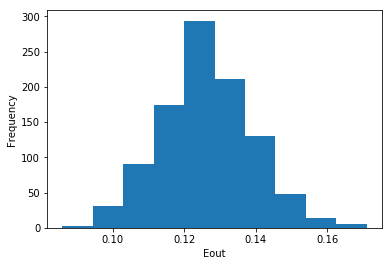
\includegraphics[scale=1]{Q7.png}
\end{figure}

\section{}
\begin{figure}[ht]
\begin{minipage}[b]{0.5\linewidth}
\centering
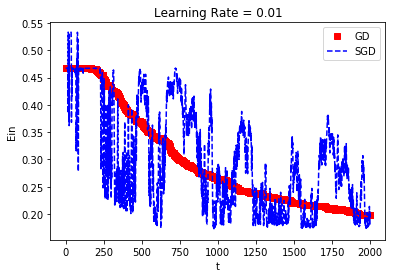
\includegraphics[scale=0.63]{Q81.png}
\end{minipage}
\hspace{0.5cm}
\begin{minipage}[b]{0.5\linewidth}
\centering
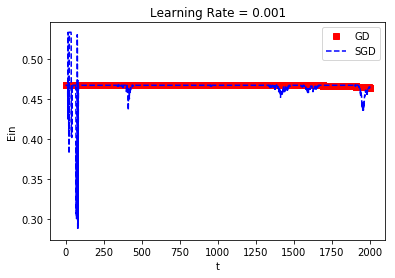
\includegraphics[scale=0.63]{Q82.png}
\end{minipage}
\end{figure}
Comparing the GD with SGD version, we can observe that the descent of error rate for GD version is more stable than SGD one's, though after 2000 iterations, their error rate could be almost the same. Moreover, it seems the fixed learning rate = 0.01 is more suitable than 0.001 since it decrease the error rate to a lower level after iterations, implying that $\eta=0.001$ may be too low steps for learning.

\section{}
\begin{figure}[ht]
\begin{minipage}[b]{0.5\linewidth}
\centering
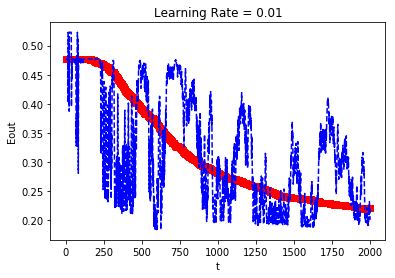
\includegraphics[scale=0.63]{Q91.png}
\end{minipage}
\hspace{0.5cm}
\begin{minipage}[b]{0.5\linewidth}
\centering
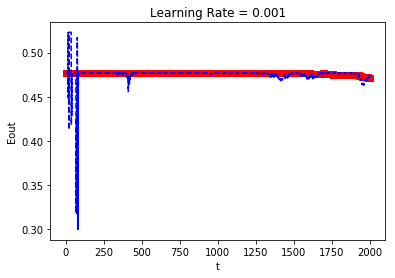
\includegraphics[scale=0.63]{Q92.png}
\end{minipage}
\end{figure}
We can find that the trend in figure Ein and Eout are almost same, which highly corresponds to what we expect: $E_{in} \approx E_{out}$. Combining with the result in previous question, we find that this algorithm achieves the learning goal.


\section{}
\begin{itemize}
 \item [(a).] We can consider the problem as solving: $\mathbf{X} \cdot \mathbf{w}_{LIN} \approx \mathbf{y}$ \\
 We want to find a vector $\mathbf{w}_{LIN}$ such that $\left \| \mathbf{X} \cdot \mathbf{w}_{LIN} - \mathbf{y} \right \| \leq \left \| \mathbf{X} \cdot \mathbf{u} - \mathbf{y} \right \| ,\forall \mathbf{u} \in \mathbb{R}^{N} $\\
 In P.15 of slides 9, we know $\left \| \mathbf{X} \cdot \mathbf{w}_{LIN} - \mathbf{y} \right \| \Leftrightarrow\mathbf{X} \cdot \mathbf{w}_{LIN}= \mathbf{H} \cdot \mathbf{y}$ , where $\mathbf{H}$ is a orthogonal projection matrix for $Col(\mathbf{X})$. \\
 \newline
 \textbf{\underline{Claim:}} $\mathbf{X}$ is a $N \times (d+1)$ matrix with $rank(\mathbf{X})=\rho$, and the SVD of $\mathbf{X}$ is $\mathbf{X}=U \Gamma V^{T}$ given in question setting, then $\mathbf{H}=U U^{T}$. \\
 Let $U U^{T}=P$, we can observe that $P^2=P^T=P$. By theorem\footnote{Suppose P is a $n \times n$ matrix such that $P^2=P^T=P$, then P is a orthogonal projection matrix for $Col(P)$. The detailed proof can be checked in Lawarence and Stephen, \textit{Elementary Linear Algebra: A Matrix Approach.}},
 we know $P$ is a orthogonal projection matrix of $Col(P)$. We want to show $Col(P)=Col(\mathbf{X})$, then $P=\mathbf{H}=U U^{T}$. \\
 First, we modify matrix $\Gamma$ by defining :
 \begin{align*}
 \Gamma^{\dagger}=\begin{bmatrix}
\frac{1}{\gamma_{1}} & 0 & 0 & \cdots & 0\\ 
 0 & \frac{1}{\gamma_{2}} & 0 & \cdots & 0\\ 
 0 & 0 & \frac{1}{\gamma_{3}} &  \cdots & 0 \\ 
 0 & 0 & 0 & \ddots & 0 \\ 
 0 & 0 & 0 & \cdots  & \frac{1}{\gamma_{\rho}}
\end{bmatrix} \text{, where we know} \; \Gamma=\begin{bmatrix}
\gamma_{1} & 0 & 0 & \cdots & 0\\ 
 0 & \gamma_{2} & 0 & \cdots & 0\\ 
 0 & 0 & \gamma_{3} &  \cdots & 0 \\ 
 0 & 0 & 0 & \ddots & 0 \\ 
 0 & 0 & 0 & \cdots  & \gamma_{\rho}
\end{bmatrix}, \gamma_{1}, \gamma_{2},...,\gamma_{\rho} > 0  \end{align*}
 It's actually easy to observe that $\Gamma^{\dagger}=\Gamma^{-1}$ , then
 \begin{align*}
  \mathbf{X}(V \Gamma^{-1} U^T) &= U \Gamma V^T V \Gamma^{-1} U^T \\
 &= U \Gamma \Gamma^{-1} U^T \\
 &= U U^T = P
 \end{align*}
 Therefore, for any vector $\mathbf{v} \in \mathbb{R}^{N}$, we have $P \cdot \mathbf{v}=\mathbf{X} \cdot \mathbf{z}$, where $\mathbf{z}= (V \Gamma^{-1} U^T) \mathbf{v}$, meaning $P \cdot \mathbf{v}$ is in $Col(\mathbf{X})$, i.e $Col(P)$ is a subspace of $Col(\mathbf{X})$. Also, $rank(P)=
 \footnote{By the property of Gramian Matrix, for any real matrix $A_{m \times n}$, $rank(A)=rank(A A^T)=rank(A^T A)$. Thus, in this question, we have $rank(U)=rank(U^T U)=rank(U U^T)=rank(I_{\rho})=rank(P)=\rho$}\rho$, i.e $dim(Col()P)=\rho$
 , then by theorem\footnote{If V and W are both the subspace of $\mathbb{R}^{n}$, and $dim(V)=dim(W)$, then $V=W$. The detailed proof can be checked in Lawarence and Stephen , \textit{Elementary Linear Algebra: A Matrix Approach }},
 $Col(P)=Col(\mathbf{X})$, hence $P=\mathbf{H}=U U^T$. \\
 \newline
 For the vector $\mathbf{w}_{LIN}$ such that $\left \| \mathbf{X} \cdot \mathbf{u} - \mathbf{y} \right \|$ is minimum, we let $\mathbf{w}_{LIN}=V \Gamma^{-1} U^T \mathbf{y}$, then $\mathbf{X} \cdot \mathbf{w}_{LIN}=\mathbf{X}(V \Gamma^{-1} U^T) \mathbf{y}= \mathbf{H} \cdot \mathbf{y}$, i.e $\mathbf{w}_{LIN}=V \Gamma^{-1} U^T \mathbf{y}$ is a solution.
 \item [(b).] Suppose there is another vector $\mathbf{s} \in \mathbb{R}^{d+1}$ can also minimize $\left \| \mathbf{X} \cdot \mathbf{u} - \mathbf{y} \right \|$ and $\mathbf{s} \neq \mathbf{w}_{LIN}$. Let $\mathbf{t}= \mathbf{s}-\mathbf{w}_{LIN}(\neq \mathbf{0})$, then 
 \begin{align*}
 \mathbf{X} \cdot \mathbf{t}= \mathbf{X} (\mathbf{s}-\mathbf{w})= \mathbf{H\cdot y- H\cdot y}= \mathbf{0} \\
 \end{align*}
Plugging SVD for $\mathbf{X}$, besides $U$ and  $\Gamma$ are invertible, we have
 \begin{align*}
 U \Gamma V^T \mathbf{t} = \mathbf{0} \\
 \Rightarrow \Gamma V^T \mathbf{t}=\mathbf{0} \\
 \Rightarrow V^T \mathbf{t}=\mathbf{0}
 \end{align*}
 Also, we know $V^T$ is a orthogonal matrix, it will reserve the inner-product.\\
 $\therefore$ $\mathbf{t \cdot w}= (V^T \mathbf{t}) \cdot (V^T \mathbf{w})=0$  \\
Now by $\mathbf{s=t+w_{LIN}}$, $\mathbf{  \left \| s \right \|^2 = \left \| t+w_{LIN} \right \|^2 = \left \| t \right \|^2 + \left \| w_{LIN} \right \|^2 > \left \| w_{LIN} \right \|^2} $, i.e $\mathbf{w}_{LIN}$ has the least norm(shortest).

\end{itemize} 


\medskip



\end{document}
